%Usually an article, 12pt font, with a seperate title page
\documentclass[12pt,titlepage]{article}
%Ability to include figures easily, and eps files
\usepackage{graphicx}
\usepackage{grffile}
\usepackage{epstopdf}
\usepackage{epsfig}
\usepackage[euler]{textgreek}
%Hide links on autoref, and call each piece a section
\usepackage[hidelinks]{hyperref}
\def\subsectionautorefname{Section}
\def\subsubsectionautorefname{Section}
%Allows symbols, captions, math
\usepackage{amssymb}
% \usepackage{amsmath} %can also use to align equations
\usepackage{caption}
%Allow acronyms, with the list beneath
\usepackage[nolist,nohyperlinks]{acronym}
\begin{acronym}
\end{acronym}
%Use natbib for bibliography
\usepackage[square,super,comma,sort&compress]{natbib}
%Style changes, indent all paragraphs, use the full page size, change the section heads, nice fractions, nice tables
\usepackage{indentfirst}
\usepackage[margin=1in]{geometry}
\usepackage{setspace}
\onehalfspacing
\usepackage[small]{titlesec}
\titlelabel{\thetitle. }
\usepackage{nicefrac}
\usepackage{booktabs}
\newcommand\tab[1][1cm]{\hspace*{#1}}
%Allows for me to non-justify some regions
\usepackage{ragged2e}

% Another package for doing title of assignment --> got it from Joel
%\usepackage{titlesec}
%\titleformat{\subsection}[runin]
%{\normalfont\large\bfseries}{\thesubsection}{1em}{}
%\titleformat{\subsubsection}[runin]
%{\normalfont\normalsize\bfseries}{\thesubsubsection}{1em}{}
\usepackage{pdflscape}
\usepackage{enumitem}% http://ctan.org/pkg/enumitem
\usepackage{adjustbox}



\begin{document}

\begin{titlepage}

\newcommand{\HRule}{\rule{\linewidth}{0.5mm}} % Defines a new command for the horizontal lines, change thickness here

\center % Center everything on the page
 
%	HEADING SECTIONS

\textsc{\LARGE McMaster University}\\[1.5cm] % Name of your university/college
\textsc{\Large MECHTRON 4TB6A}\\[0.5cm] % Major heading such as course name
\textsc{\large Mechatronics \& Software Engineering Capstone}\\[0.5cm] % Minor heading such as course title

%	TITLE SECTION
\vspace{1cm}
\HRule \\[0.2cm]
{ \Large \vspace{0.25cm}  \textsc{  \LARGE Hazard Analysis } \vspace{0.3cm} }  % Title of your document
\HRule \vspace{1cm}

\textsc{\LARGE Health Mate - Pill Dispenser}
 
 \begin{figure}[h]
  \centering
  
\includegraphics[width=.4\linewidth]{../ApexEngineering.png}
\end{figure}
 \vspace{1cm}
 
%----------------------------------------------------------------------------------------
%	AUTHOR SECTION
%----------------------------------------------------------------------------------------

\begin{table}[ht!]
\centering
\begin{tabular}{c c c}
\toprule
\textbf{Name} & \textbf{Student Number} & \textbf{McMaster Email}         \\ \midrule
Justin Ballaro & 400015482 & ballaroj@mcmaster.ca \\
Joel Bates & 001420696 & batesjj@mcmaster.ca \\
Brodie Bresette & 400029059 & bresettb@mcmaster.ca \\
Nicholas D'Angelo & 400018631 &  dangelon@mcmaster.ca  \\
Daniel Pietrangelo & 400010287 &  pietrand@mcmaster.ca \\
  \bottomrule
\end{tabular}
\label{Tab:HU}
\end{table}

%	DATE SECTION
\vfill
{\large Sunday, December 27, 2020}\\[3cm] % Date, change the \today to a set date if you want to be precise
 % Fill the rest of the page with whitespace

\end{titlepage}

\pagebreak
\pagenumbering{roman}
\tableofcontents
\pagebreak
\pagenumbering{arabic}

\section{Table of Revisions}

\begin{table}[ht!]
\begin{center}
\begin{adjustbox}{max width=\textwidth}
\small
\begin{tabular}{|p{0.1\textwidth}|p{0.1\textwidth}|p{0.2\textwidth}|p{0.4\textwidth}|}
 \hline
 \textbf{Revision } & \textbf{Date} &
 \textbf{Authors} &
 \textbf{Revision Comments}\\
 \hline \centering
 0 & \centering
 12/27/2020 & 
 Justin Ballaro \newline
Joel Bates \newline
Brodie Bresette \newline
Nicholas D'Angelo \newline
Daniel Pietrangelo &
Initial Revision \\
\hline
\end{tabular}
\end{adjustbox}
\end{center}
\caption{Table of Revisions}
\end{table}

\pagebreak

\section{Introduction}
\subsection{Scope of Project}
The desired system shall automate the dispensing of a person's medication from a standard sized pill blister back that is inserted by the user. This dispensing shall occur at times set by the user within the specified ranges of the pill blister pack (Morning, Afternoon, Evening, Night). The device shall also collect dispensing statistics for review by the user along with any other health professional. 

\subsection{Scope of Document}
The scope of this document is to outline potentially hazardous issues that could result from the pill dispenser's subsystems. More specifically, this document will outline hazardous scenarios that may result from the hardware and software subsystems. 

The issues outlined in this document will be documented from cases where the device is considered to be working correctly as well as working incorrectly. Also, hazards that could potentially evolve from the development of this device will be analyzed and included in this report. This analysis should be conducted throughout the development life cycle of the device. 



\section{System Overview}
\subsection{Scheduling System}
This system allows the user to set a dispensing time for each dispensing period (Morning, Afternoon, Evening, Night).
\subsection{Notification System}
The device's notification system will alert the user when the time has been reached to take their scheduled medication. This includes an audible alarm, along with other measures yet to be defined.
\subsection{Loading System}
This system will allow the user to load the desired blister pill pack into the device.
\subsection{Calibration System}
The calibration system will ensure the blister pill pack is loaded properly into the device, all system parameters are set correctly and the dispensing mechanism is in working order. 
\subsection{Dispensing System}
The dispensing system for the device will perform the required motion to break open the blister allowing the pills to be removed from the pack and be dispensed by the device. This system also includes the mechanism for pill retrieval.
\subsection{Data Collection System}
Data collection for the device will involve collecting on-board sensor data to retrieve metrics on medication adherence and device use. 

\section{Safety Considerations}
\subsection{Scheduling System}
\subsubsection*{Software Issues}
\begin{itemize}
\item Schedule file corruption during saving or loading to/from device.
\item Scheduling system timing configuration may not match the time used on the device. This may cause conflict of timing between the device and schedule.
\item Dispensing time scheduled that is outside allowable range of values.
\item Previously inputted schedule could be lost due to override of new schedule.
\end{itemize}
\subsubsection*{Hardware Issues}
\begin{itemize}
\item Mechanism for user input malfunctions (faulty connection, mechanical failure of button/switch).
\item Display used to set schedule malfunctions.
\end{itemize}

\subsection{Notification System}
\subsubsection*{Software Issues}
\begin{itemize}
\item Notification signal is not sent/is sent at the wrong time (in accordance with scheduling system).
\item Notification signal is not terminated once pills are retrieved from the device.
\item Notification signal is terminated before pills are retrieved or before time-out duration is reached.
\end{itemize}
\subsubsection*{Hardware Issues}
\begin{itemize}
\item Alarm/Speaker stops working or burns out.
\item If accuracy or reliability of on-board RTC is not sufficient, notifications may not be triggered.
\item Button used to terminate the alarm stops working.
\end{itemize}

\subsection{Loading System}
\subsubsection*{Software Issues}
\begin{itemize}
\item \textbf{\item Device may not detect if blister pack is `locked'.}
\end{itemize}
\subsubsection*{Hardware Issues}
\begin{itemize}
\item Loading system may lock/unlock during device processes when it is not needed.
\item Blister pack becomes damaged during insertion/removal by user. 
\item Blister pack is loading into the device in the wrong orientation.
\item Dispensing mechanisms get stuck, preventing the insertion or removal of blister packs.
\end{itemize}

\subsection{Calibration System}
\subsubsection*{Software Issues}
\begin{itemize}
\item Calibration signal is not received from hardware.
\item Read success signal when calibration fails or failure signal when calibration succeeds.
\end{itemize}
\subsubsection*{Hardware Issues}
\begin{itemize}
\item Limit switches become stuck.
\item Limit switch is not sending electrical signal (loose connection, faulty parts)
\item Dispensing mechanism damages limit switch.
\end{itemize}

\subsection{Dispensing System}
\subsubsection*{Software Issues}
\begin{itemize}
\item System does not dispense medication at the scheduled time.
\item Signal to dispense is sent to system when a blister pack is not loaded into the device.
\item Signal to dispense is sent to system before a successful calibration has taken place.
\end{itemize}
\subsubsection*{Hardware Issues}
\begin{itemize}
\item Stepper motor not functioning properly, not ending in the proper location.
\item Failure to sense when blister is broken and pills have been dispensed.
\item System identifies a successful dispense despite their being a failure.
\item Manual dispensing button malfunctions.
\item Insufficient power transferred from motor to actuators and piercers.
\item Linear actuators break/becomes stuck. 
\item Blister piercer breaks/malfunctions.
\item Blister piercer damages pills.
\item Pills become stuck/damaged while falling into collection bay.
\item Dispensed pills bounce of out collection bay.
\item Device does not return to safe state after an unexpected power outage.
\item Unexpected obstacles preventing regular motion of motors and linear actuator.
\end{itemize}

\subsection{Data Collection System}
\subsubsection*{Software Issues}
\begin{itemize}
\item Corruption of data when saving/loading to and from device.
\item Failure to record taken and missed medication doses.
\item False negative and false positive data is recorded for taken/missed dose.
\item Failing to write data into non-volatile memory.
\end{itemize}
\subsubsection*{Hardware Issues}
\begin{itemize}
\item Issues preventing read/write operations between micro-controller and memory.
\end{itemize}

\pagebreak
\section{Failure Modes and Effect Analysis Table}


\begin{figure}[!htbp]
    % \centering
    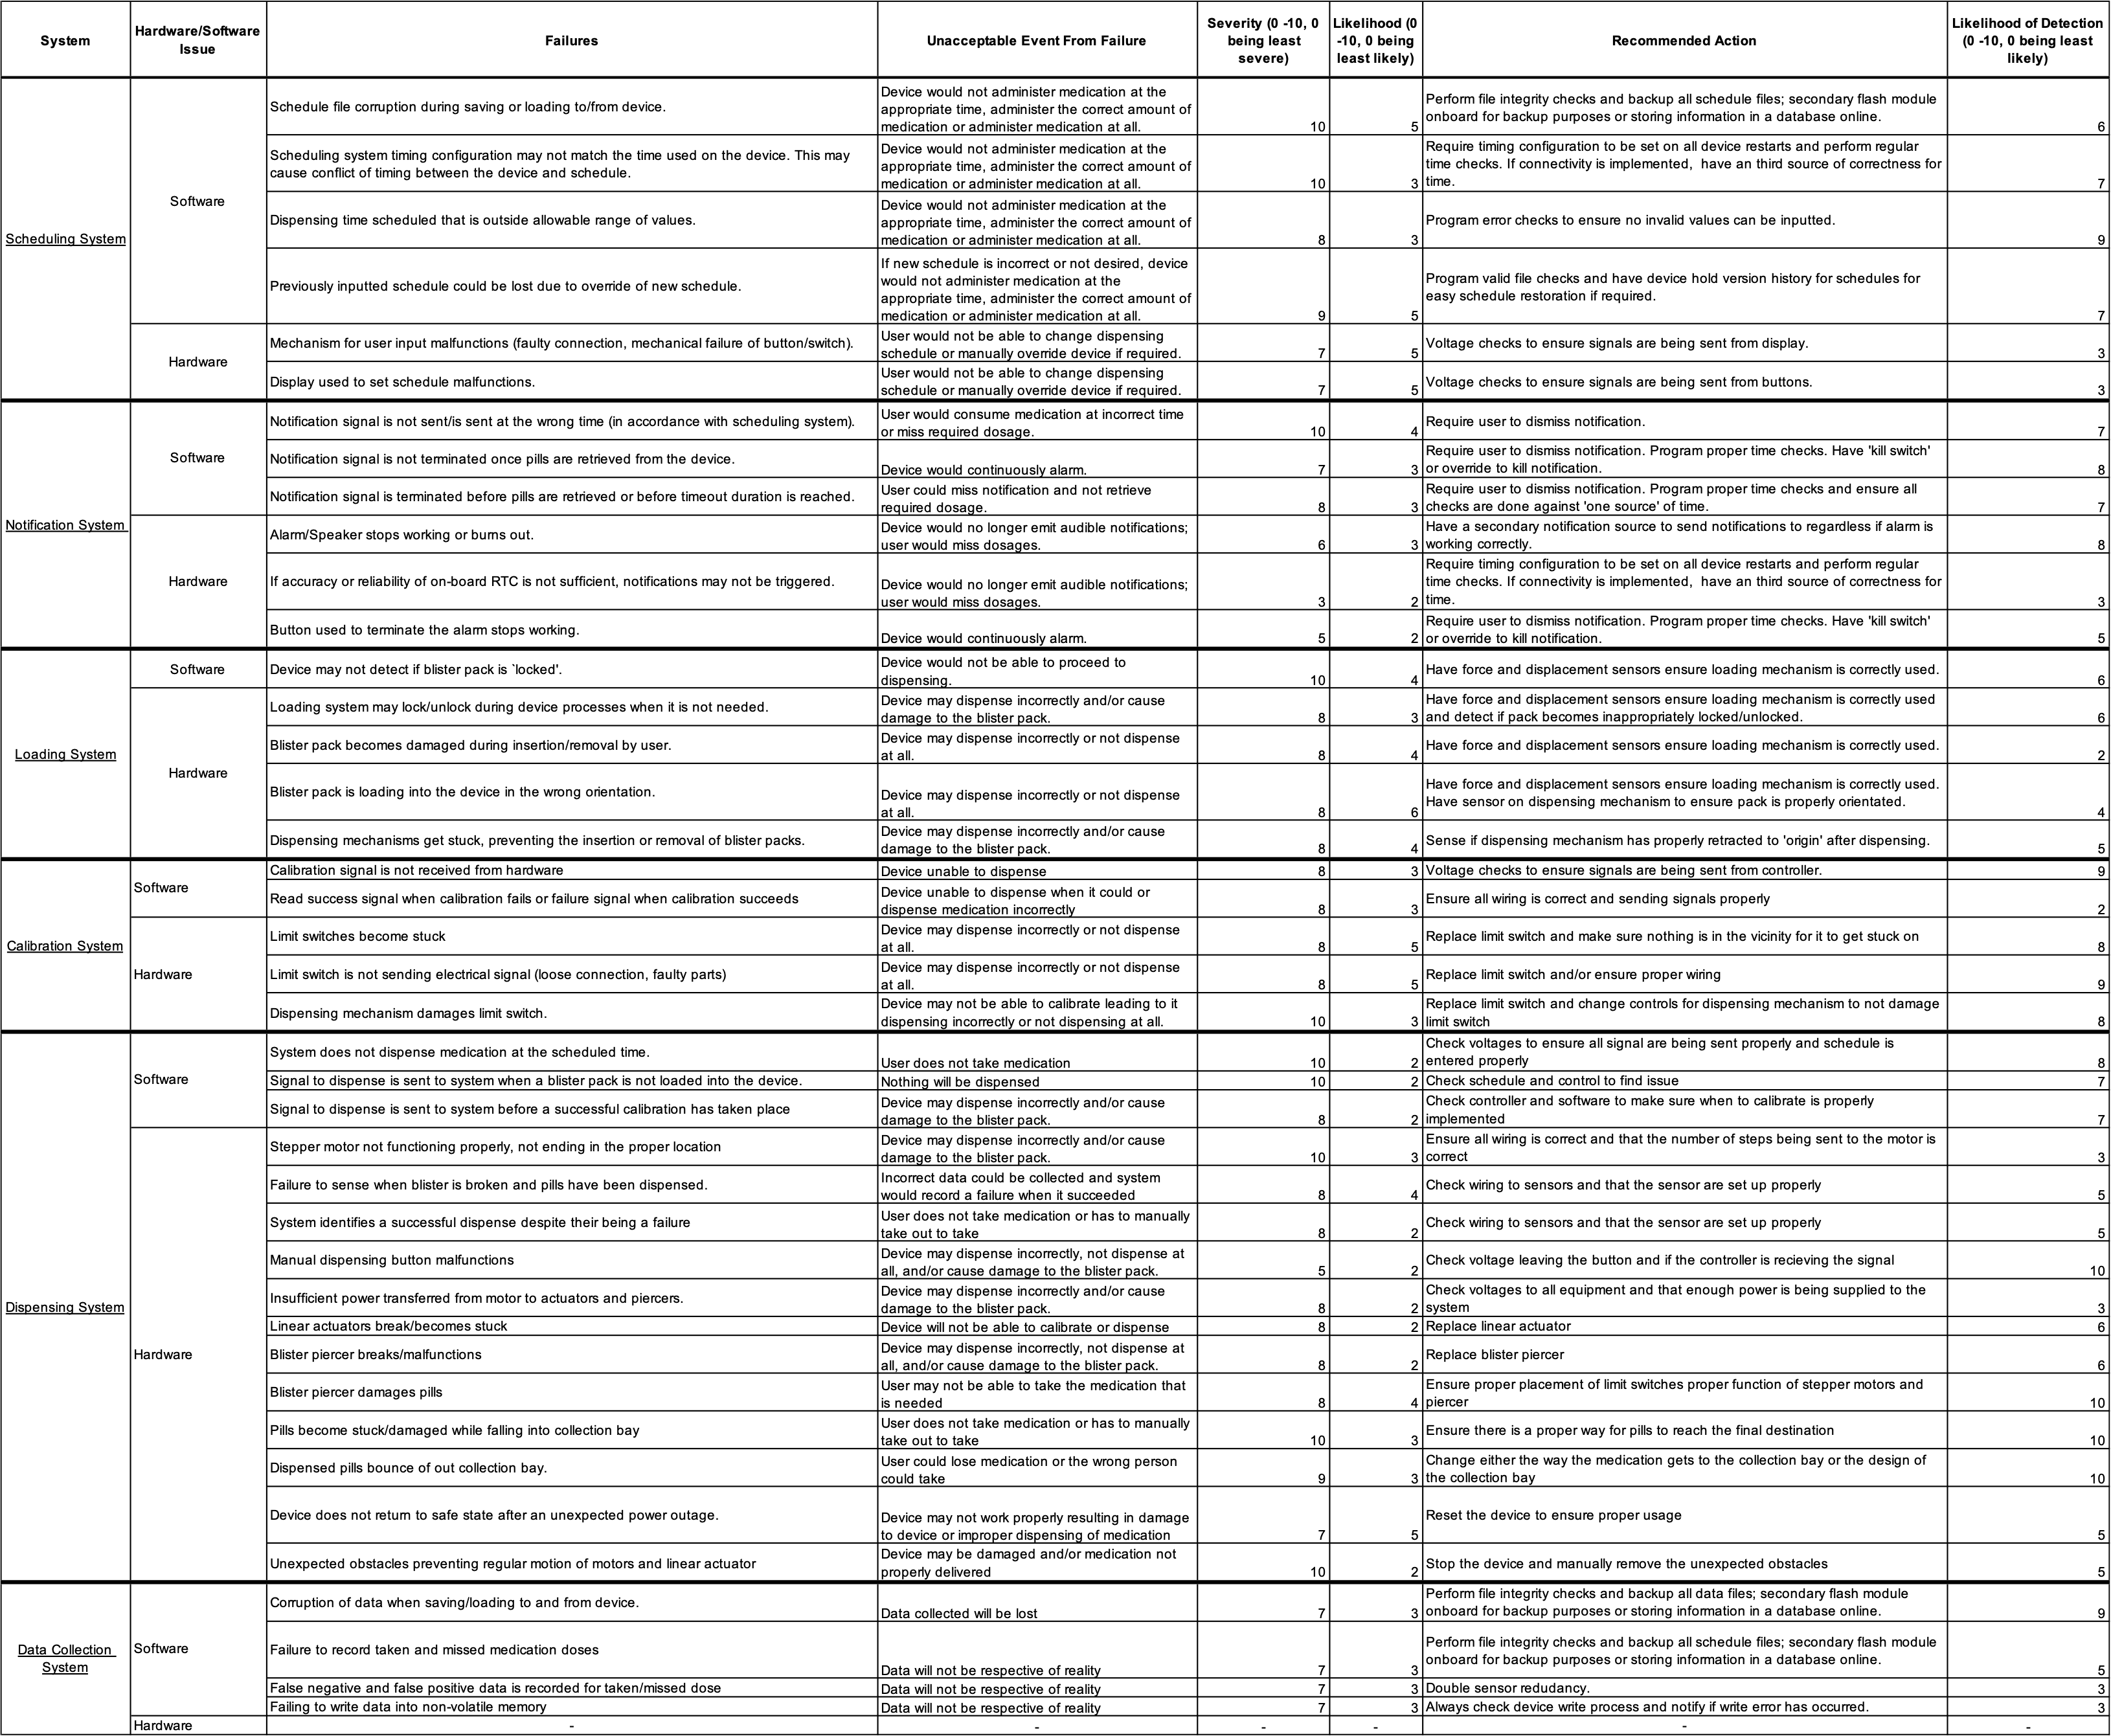
\includegraphics[width=\textwidth,height=\textheight,keepaspectratio]{./fmea.png}
    \caption{FMEA Table}
    \label{fig:my_label}
\end{figure}



\end{document}